\documentclass[12pt]{article}

% packages
\usepackage[margin=1in]{geometry}
\usepackage{graphicx}
%\usepackage{subcaption}  % needed for sub figures
\usepackage{enumerate}
\usepackage{paralist}
\usepackage{xcolor}
\usepackage[hypcap]{caption}
%\usepackage[pdftex, colorlinks=true, linkcolor=blue]{hyperref}		% comment in final draft
\usepackage[colorlinks=false,urlbordercolor=white]{hyperref}

\usepackage[sort&compress,numbers]{natbib}
\usepackage{wrapfig}
\usepackage{subfig}


% Fonts
\usepackage[T1]{fontenc}
%\usepackage{lmodern}
\usepackage{mathptmx}
%\usepackage{fourier}
%\usepackage{tgtermes}
%\usepackage{cmbright}
%\linespread{1.1}

%%%%%%%%%%%%%%%%%%%%%%%%%%%%%%%%%%%%%%%%%%%%%%%%%%%%%%%%%%%%%%%%%%%%%%%%
% Formatting for DARPA report
%\usepackage{titlesec}
%\titleformat{\section}[runin]{\normalfont\normalsize\bfseries}{\thesection.}{1em}{}

%% indenting
%\usepackage{indentfirst}

\usepackage{titlesec}
\titleformat*{\section}{\normalsize\bfseries}
%\titleformat*{\subsection}{\normalsize\bfseries}
%\titleformat*{\subsubsection}{\normalsize\bfseries}

\titleformat{\subsection}
{\normalfont\normalsize\bfseries}{\thesubsection}{1em}{}
\titlespacing*{\subsection}{\parindent}{3.25ex plus 1ex minus .2ex}{1.5ex plus .2ex}

\titleformat{\subsubsection}[runin]
{\normalfont\normalsize\bfseries}{\thesubsubsection}{1em}{}
\titlespacing*{\subsubsection}{\parindent}{3.25ex plus 1ex minus .2ex}{1.5ex plus .2ex}


%\newcounter{DarpaSecCounter}
%\setcounter{DarpaSecCounter}{0}
%%\newcommand{\rsection}[1]{\stepcounter{DarpaSecCounter}\vspace{15pt}\noindent\textbf{{\theDarpaSecCounter.} #1}\vspace{3pt}}
%\renewcommand{\section}[1]{\stepcounter{DarpaSecCounter}\vspace{15pt}\noindent\textbf{{\theDarpaSecCounter.} #1}\vspace{3pt}}
%
%
%\newcounter{DarpaSubSecCounter}[DarpaSecCounter]
%%\setcounter{DarpaSubSecCounter}{1}
%%\newcommand{\rsubsection}[1]{\stepcounter{DarpaSubSecCounter}\indent\textbf{\theDarpaSubSecCounter. #1}}
%\renewcommand{\subsection}[1]{\vspace{4pt}\stepcounter{DarpaSubSecCounter}\indent\textbf{\theDarpaSecCounter.\theDarpaSubSecCounter. #1.}}
%
%\newcounter{DarpaSubSubSecCounter}[DarpaSubSecCounter]
%\renewcommand{\subsubsection}[1]{\vspace{2pt}\stepcounter{DarpaSubSubSecCounter}\indent\textbf{\theDarpaSecCounter.\theDarpaSubSecCounter.\theDarpaSubSubSecCounter.} \emph{#1}}

%%%%%%%%%%%%%%%%%%%%%%%%%%%%%%%%%%%%%%%%%%%%%%%%%%%%%%%%%%%%%%%%%%%%%%%%


\usepackage{amsmath}
\usepackage{amsthm}
\usepackage{amsfonts}
\usepackage{amssymb}
%\usepackage{mathrsfs}  % nice script fonts
\usepackage{mathtools}
\usepackage{bm} % bold math
%\usepackage{bbm} % blackboard math \mathbbm
%\usepackage{stix}



% Quick math font modification
\newcommand{\mc}{\mathcal}
\newcommand{\msf}{\mathsf}
%\newcommand{\mbf}{\bm} 			% requires amsmath, amssymb packages
\newcommand{\mbf}{\mathbf}            % requires amsmath, amssymb packages
\newcommand{\mbb}{\mathbb}    % requires bbm
\newcommand{\mf}{\mathfrak}
\newcommand{\mscr}{\mathscr}

% Spaces
\newcommand{\N}{ \ensuremath{\mathbb{N}}}  % natural numbers
\newcommand{\Z}{ \ensuremath{\mathbb{Z}}}  % integers
\newcommand{\Q}{ \ensuremath{\mathbb{Q}}}
\newcommand{\R}{ \ensuremath{\mathbb{R}}}  % real numbers
\newcommand{\C}{ \ensuremath{\mathbb{C}}}  % complex numbers
\newcommand{\K}{ \ensuremath{\mathbb{K}}}  % scalar field \R or \C
\newcommand{\T}{\ensuremath{\mathbb{T}}}
\newcommand{\D}{ \ensuremath{\mathbb{D}}}

% Short-hand greek
\newcommand{\eps}{\epsilon}
\newcommand{\del}{\delta}
\newcommand{\lam}{\lambda}
\newcommand{\al}{\alpha}

% set theory
\providecommand\given{} % make sure it exists
\newcommand\SetSymbol[1][]{
\nonscript\,#1\vert \allowbreak \nonscript\,\mathopen{}}

\DeclarePairedDelimiterX\set[1]{\lbrace}{\rbrace}{ \renewcommand\given{\SetSymbol[\delimsize]} #1 }  % set* autoscales
\newcommand{\Union}{\bigcup}        % big union
\newcommand{\union}{\cup}            % little union
\DeclareMathOperator{\inter}{int}

% Vector spaces/ Operators
\DeclarePairedDelimiterX\norm[1]{\lVert}{\rVert}{#1}            % norm (\norm*{} autoscales or \norm[\big]{})
\DeclarePairedDelimiterX\inner[2]{\langle}{\rangle}{#1 \,,\, #2}    % inner product
\newcommand{\transp}{\mathsf{T}}                                % transpose
\DeclareMathOperator{\linspan}{span}                            % linear span
\DeclareMathOperator{\rank}{rank}                                % Rank of a matrix.
\DeclareMathOperator{\diag}{diag}                                % Diagonal matrix.
\newcommand{\Null}{N}                                            % Nullspace
\newcommand{\Ran}{Ran}                                            % Range
\DeclareMathOperator{\image}{Im}                                % Image
%\newcommand{\closure}[1]{\overline{#1}}							% Closure

% math functions
\DeclarePairedDelimiterX\abs[1]{\lvert}{\rvert}{#1} % absolute value: \abs{} = no-resize, \abs*{} = left/right auto-resize, \abs[size-cmd]{} = size manually adjusted with size-cmd = \big,\Big,\bigg,\Bigg
\DeclareMathOperator{\sign}{sgn}
\newcommand{\one}{ \ensuremath{\bm{1}}}
\DeclareMathOperator{\supp}{supp}                                % Support
%\newcommand{\ind}[1]{\mathbb{I}_{#1}}							% indicator function
\newcommand{\ind}[1]{\mathbbm{1}_{#1}}                            % indicator function
\newcommand{\ud}{\,d}  % differential with space before symbol

% Theorem environments
\theoremstyle{plain}
\newtheorem{theorem}{Theorem}[section]
\newtheorem{lemma}[theorem]{Lemma}
\newtheorem{proposition}[theorem]{Proposition}
\newtheorem{conjecture}[theorem]{Conjecture}
\newtheorem{claim}[theorem]{Claim}
\newtheorem{myquestion}[theorem]{Question}
\newtheorem*{corollary}{Corollary}
\theoremstyle{remark}
\newtheorem*{remark}{Remark}
\newtheorem*{remarks}{Remarks}
\newtheorem*{justification}{Justification}
\theoremstyle{definition}
\newtheorem{example}[theorem]{Example}
\newtheorem{definition}[theorem]{Definition}
\newtheorem*{notation}{Notation}


% annotate
\newcommand{\blue}[1]{{\color{blue} #1}}
\newcommand{\red}[1]{{\color{red} #1}}
\newcommand{\needcite}{{\tiny\blue{need citation}}}
\newcommand{\todo}[1]{{\tiny\red{#1}}}

% paper-specific definitions
\newcommand{\mat}[1]{\mbf{#1}}  % font style for matrices
\newcommand{\op}[1]{\mathcal{#1}}  % font style for operators
\newcommand{\vsp}[1]{\mathsf{#1}}  % font style for vector spaces
\newcommand{\size}[1]{\mathrm{size}(#1)}
\newcommand{\up}{\uparrow}
\newcommand{\dn}{\downarrow}

\newcommand{\Ko}{C}  % Koopman operator
\newcommand{\Kdm}{A}  % Koopman diffusion operator (asymmetric kernel)
\newcommand{\Dm}{D}  % Diffusion operator (symmetric kernel)
\newcommand{\psdm}{p_{\sigma,\delta}^{(m)}}

\usepackage{lipsum}

\renewcommand{\r}{\bm{p}}
\newcommand{\units}[1]{\mathsf{#1}}


\newcommand{\bmat}[1]{\begin{bmatrix}
                          #1
\end{bmatrix}} % short hand bracket matrix
\newcommand{\pmat}[1]{\begin{pmatrix}
                          #1
\end{pmatrix}} % short hand bracket matrix

\newcommand{\rmm}[1]{{\color{red}#1}}

\renewcommand{\vec}[1]{\mathbf{#1}}

\newcommand{\x}{\mathbf{x}}

\newcommand{\email}[1]{\href{mailto:#1}{\color{blue}\underline{#1}}}

% MHG packages
\usepackage[version=3]{mhchem}
\usepackage{braket}
\usepackage{relsize}
%\usepackage{enumitem}
%\usepackage[vlined]{algorithm2e}
%\usepackage{algpseudocode}
%\usepackage[font=small,labelfont=bf]{caption}
%\usepackage{graphicx}
%\usepackage{footnote}
%\usepackage{multirow}
%\usepackage{tabularx}
\usepackage{booktabs}
\usepackage{makecell}
\usepackage{threeparttable}
\usepackage{chemfig}
\usepackage{siunitx}

%========================================================================
\begin{document}

    %========================================================================

    % == Accomplishments during reporting period
    \section[Intro]{Introduction}
    \label{sec:intro}
    Partial Differential Equations (PDE) are fundamental to model different phenomena in science and engineering
    mathematically.
    Previous methods have shown strong performance in approximating the solutions of PDEs using Deep Neural Networks
    (DNN) [https://arxiv.org/pdf/1908.10407.pdf].
    In this work, we approximate the PDE of dynamical systems using only symmetry constrained observations of the
    target system.

    \section{Background}
    \label{sec:background}
        \subsection{PDE}
        \subsection{DNN}




    \section{Executive summary}

    We discovered a new method of approximating partial differential equations using deep neural networks. These methods are able to predict turbulent flow as effectively as previous methods without relying on complex memory gates instead using an approximate form of partial differential equations (PDEs). Additionally, by nature of approximating an arbitrary PDE, solutions fit a powerful class of equations capable of modeling many physically based systems.

    \subsection{Formulating Approximation of Partial Differential Equations}

    \subsubsection{What was to be tested? What was the expected outcome prior to testing?}
    Previous results used sequence-to-sequence models to learn an embedding of the current state, as well as a model of the dynamics using recurrent networks such as Long-Short Term Memory units (LSTMs). This worked well for prediction, however recurrent neural networks represent a much more complex function approximation scheme. While RNNs have been shown to approximate dynamical systems [Sonoda \& Murata (2017)], complex and non-linear mechanics such as forget-gates do not map well to the discovery of physical laws.

    \subsubsection{High-level summary of main results.}
    Explicitly modeling the dynamics as a PDE allows for interpolation by adjusting $\bigtriangleup t$ in the discretized time derivative. Additionally, because many physically based systems are easily modeled using PDEs, the class of problems is well understood and forms a basis for many natural processes such as diffusion, electrostatics, or fluid dynamics.

    \subsubsection{Discuss relevance to project and DARPA concerns.}
    This formulation moves previous models towards more explainable and better understood formulations simultaneously reducing the number of learned parameters in the model. Solutions that offer good representation using this scheme can be more easily reasoned about and require fewer calculations to infer.

    \subsection{Evaluating Predictions of Approximated Partial Differential Equations}

    \subsubsection{What was to be tested? What was the expected outcome prior to testing?}
    We evaluate new approximate PDE based architecture against the previous recurrent model over different sequence lengths comparing against the best LSTM based architecture found previously.


    \subsubsection{High-level summary of main results.}
    Despite a reduction in complexity as well as strong spacial assumptions, the newly discovered architecture performs almost as well as the previous optimized model. Preliminary experiments already achieve a MSE of 0.0023 compared to an optimized MSE of 0.0016 from the best performing LSTM model over 20 time steps. Further results suggest that the assumption of spacial uniform dynamics is significantly impacting prediction, with a short, 5 step model achieving an excellent MSE of 0.000069, an improvement of over 95\% compared to the best LSTM model.

    \subsubsection{Discuss relevance to project and DARPA concerns.}
    These results show the new architecture is capable of predicting turbulent flow effectively, even when given fewer frames of history. Moreover, there is strong potential for further model improvements. Thus we maintain previous successes with predicting turbulent flow while simplifying the network architecture.

    %========================================================================
    \section{Achievements}

    \subsection{Scientific Breakthroughs}

    None

    \subsection{Technology developments}

    None

    \subsection{Application results}

    More work is needed to determine if the discovered formulation is well suited for applications in sequence interpolation.

    \subsection{Transitions achieved}

    None

    %========================================================================
    \section{Lessons Learned}

    \noindent

    \noindent Problems encountered/risks that occurred, and corresponding solutions/mitigations

    \noindent Open Issues

    %========================================================================
    \section{Next Steps}

    \noindent Incorporating local features in the dynamics model is necessary to correctly approximate partial derivatives, however, as the dynamics model is uniform across the entire domain, strong edge effects distort the dynamics. Developing a model capable of overcoming edge effects will allow the dynamics to more robustly rely on local features and could dramatically improve performance.


    \noindent Current scheme uses only a single time derivative to approximate the dynamics. By incorporating higher order approximations, more information can be captured in the learned PDE.

    \noindent The current formulation learns a discretized time derivative of the dynamics. If model is capable of interpolating between intermediate samples, this would be invaluable for both data compression and super-sampling sequences.

    \noindent Previous formulations were robust to noise and missing samples. Following this work, we will compare noise resistance of the new fully convolutional formulation against the previous recurrent LSTM based model.

    %========================================================================
    \section{Technical details}

    \subsection{Formulating Approximation of Partial Differential Equations}

    \begin{figure}
        \centering
        \begin{minipage}[c]{\textwidth}
            \centering
            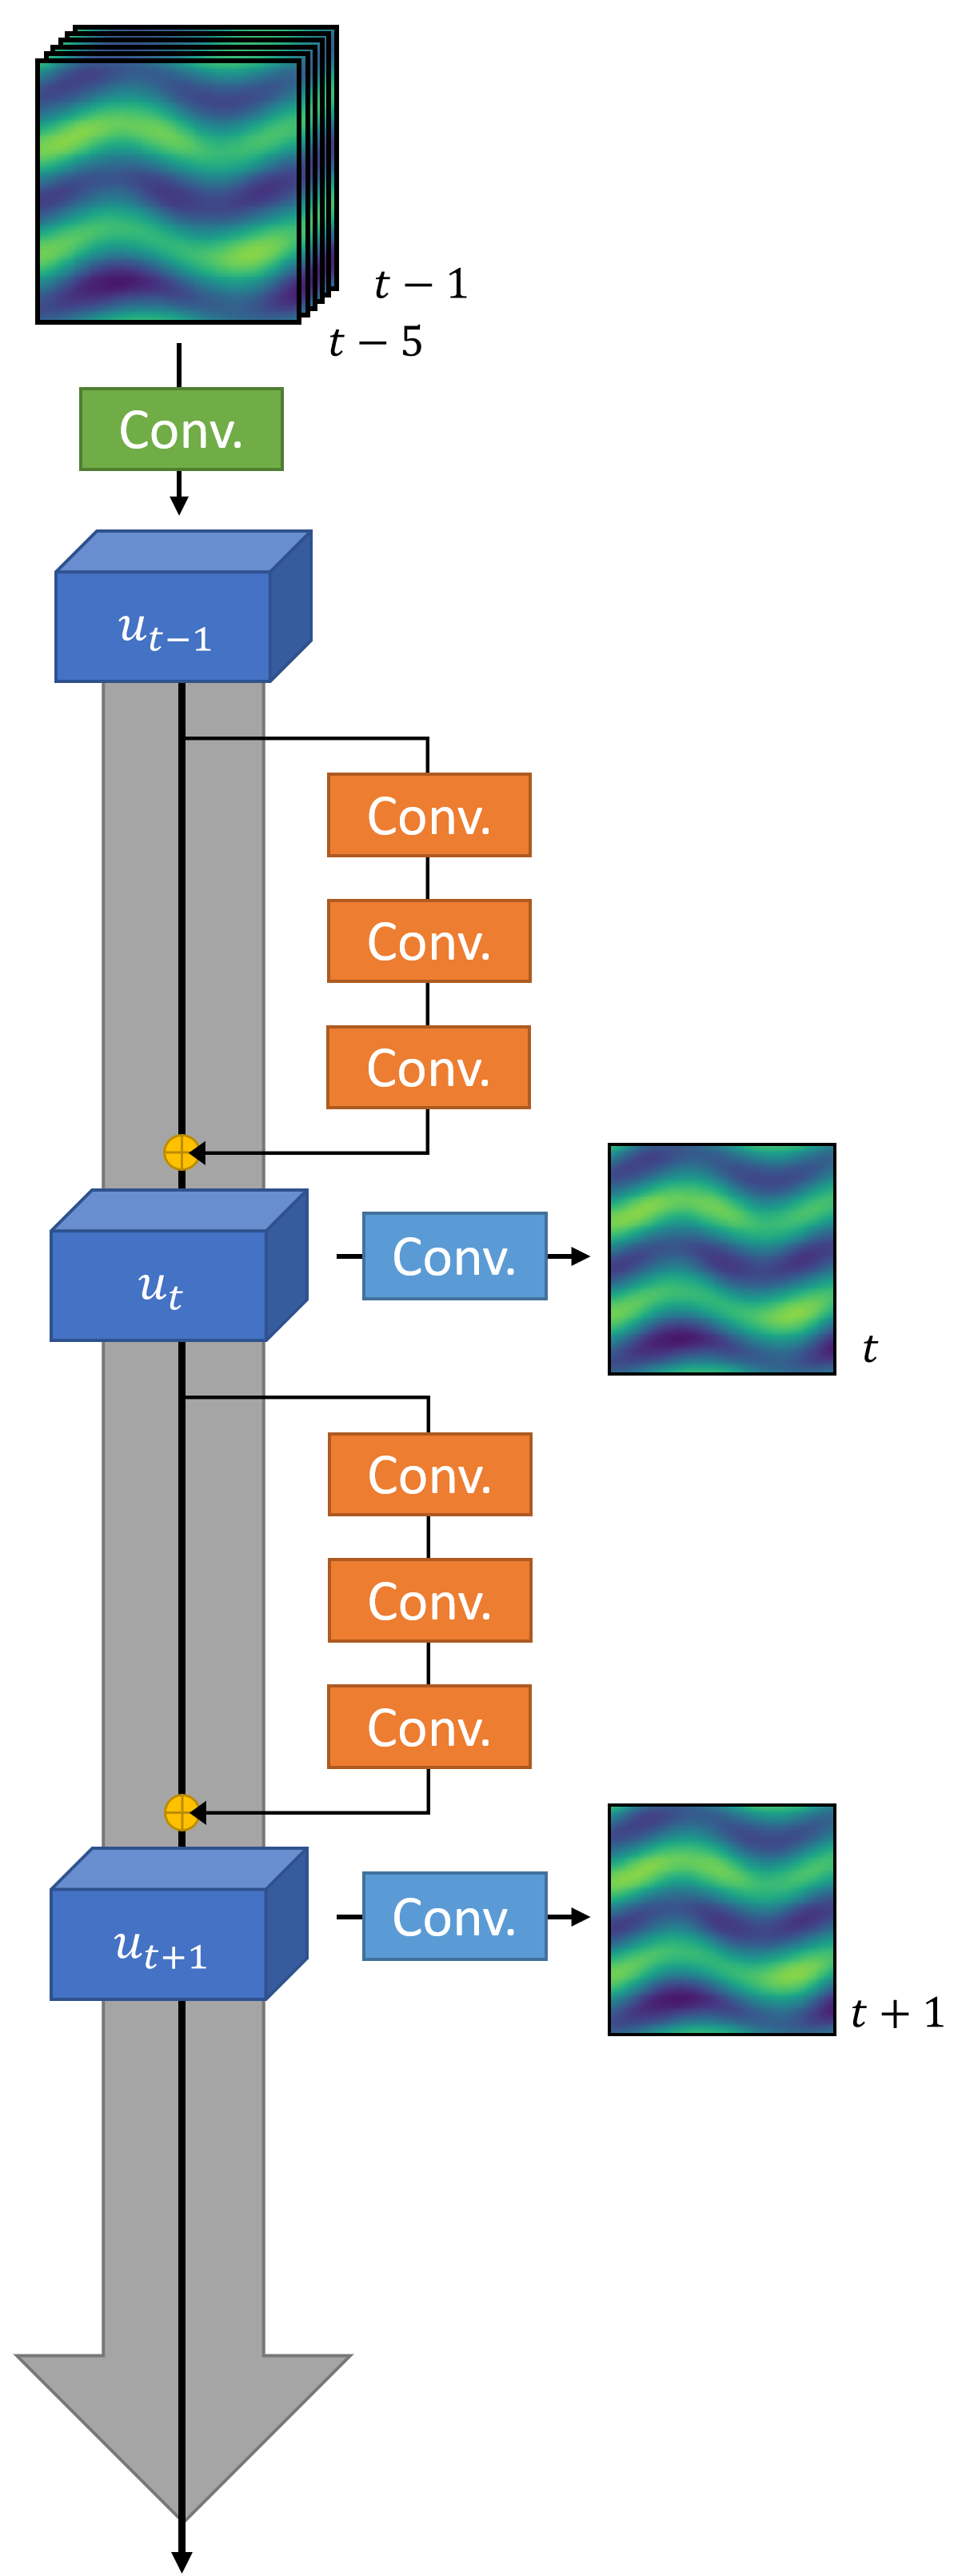
\includegraphics[width=2.5in]{pde_arch}
            \caption{Illustration of the res-net inspired forward Euler architecture. The encoder $\phi(x)$ (shown in green) maps the input into the feature space. Three sequential convolutional layers (shown in orange) are used to approximate $f(u_n)$ and summed with $u_n$ (shown in yellow) to give $u_{n+1}$ as outlines in equation \ref{eqn:ode}. At each step, the feature vector $u_n$ is decoded by $\theta(u_n)$ (as shown in light blue) predicting $x_n$. }
            \label{fig:pdearch}
        \end{minipage}
    \end{figure}


    Consider learning a PDE of the form $u_t = f(u)$. The simplest approximation of $u_t = f(u)$ is to discretize the time derivative $u_t$ by $\frac{u_{n+1} - u_n}{\bigtriangleup t}$ and approximate the right hand side by $f(u_n)$. This leads to the forward Euler scheme

    $$u_{n+1} = u_n + \bigtriangleup t f(u_n) \label{eqn:ode} $$

    where $f(u_n)$ is learned by a deep neural network. Instead of learning the dynamics of the system directly, we use a learned feature representation $u_n$ composed of linear convolutions of the input history. This avoids the need for approximating the local partial derivatives of the system and instead allows the network to learn the optimal feature representation.


    Let $x$ represent h patches of history $x = [x_{t-h}, ..., x_{t-1}]$ and y represent the target sequence $y =
    [x_{t}, x_{t+1},...,x_{t+l-1}]$. We learn an encoder, $\phi(x) = u_0$, a decoder $\theta(u_n) = \hat{x}_n$ as well as a dynamics model $f(u_n)$ from equation \ref{eqn:ode}.

    We utilize a feature space of dimension m = 16, therefore $u_n \in \R^{16}$. Additionally, to ensure spatial continuity, we expand the domain of  $f(u_n)$ to include the local 5x5 region centered about each pixel of a given patch, thus $f(u_n) \in \R^{16 \times 5 \times 5}$ $\rightarrow \R^{16}$.
    Similarity for the encoder, we introduce local features by convolving 16 filters of shape 5x5x5 giving us $\phi(x) \in \R^{5*5*5} \rightarrow \R^{16}$. Finally, for the decoder $\theta(u_n)$ we simply apply a reduction over the feature space, giving  $\theta(u_n) \in \R^{16} \rightarrow \R$

    % Thus we learn a series of features $w_{enc}$ such that $u_0 = relu(x * w_{enc})$.
    % We approximate the dynamics $f(u)$ by    $f(u_n)$ by

    % us to learn the dynamics of a system by approximate the dynamics of these features in the system by $f(u_n)$ by


    \subsection{Evaluating Predictions of Approximated Partial Differential Equations}

    \begin{figure}
        \begin{minipage}[t]{0.45\linewidth}
            \centering
            
\includegraphics[width=0.7\linewidth]{pde_prediction}
            \caption{Mean absolute error over a single validation batch for PDE architecture. Because of the strong spatially invariant assumptions made by the model, we see strong edge effects near the borders. }
            \label{fig:pdeprediction}
        \end{minipage}
        \begin{minipage}[t]{0.1\linewidth}
            \centering
            \hspace{1\linewidth}
        \end{minipage}
        \begin{minipage}[t]{0.45\linewidth}
            \centering
            
\includegraphics[width=0.7\linewidth]{lstm_prediction}
            \caption{Mean absolute error over a single validation batch for LSTM architecture. Note the error is more uniform through the entire patch. }
            \label{fig:lstmprediction}
        \end{minipage}
    \end{figure}


    \begin{figure}
        \centering
        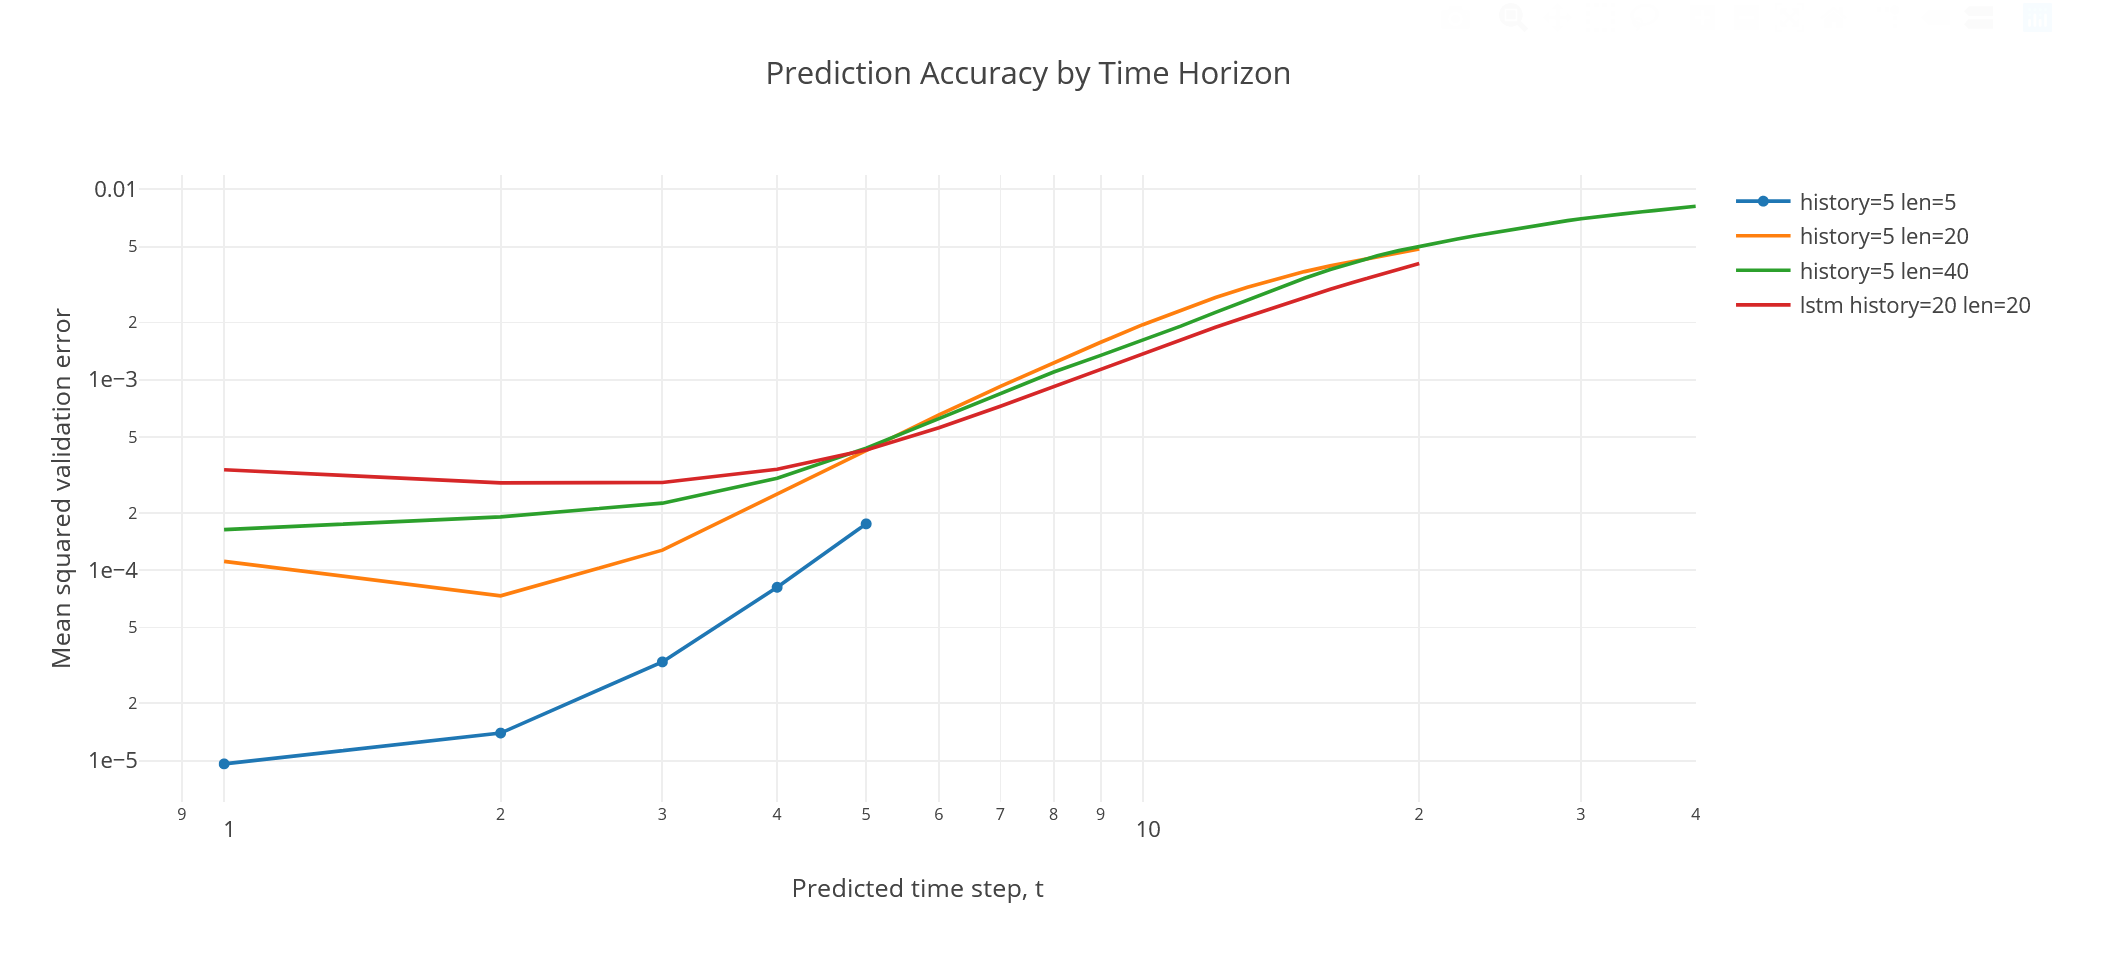
\includegraphics[width=0.9\linewidth]{pde_perf}
        %	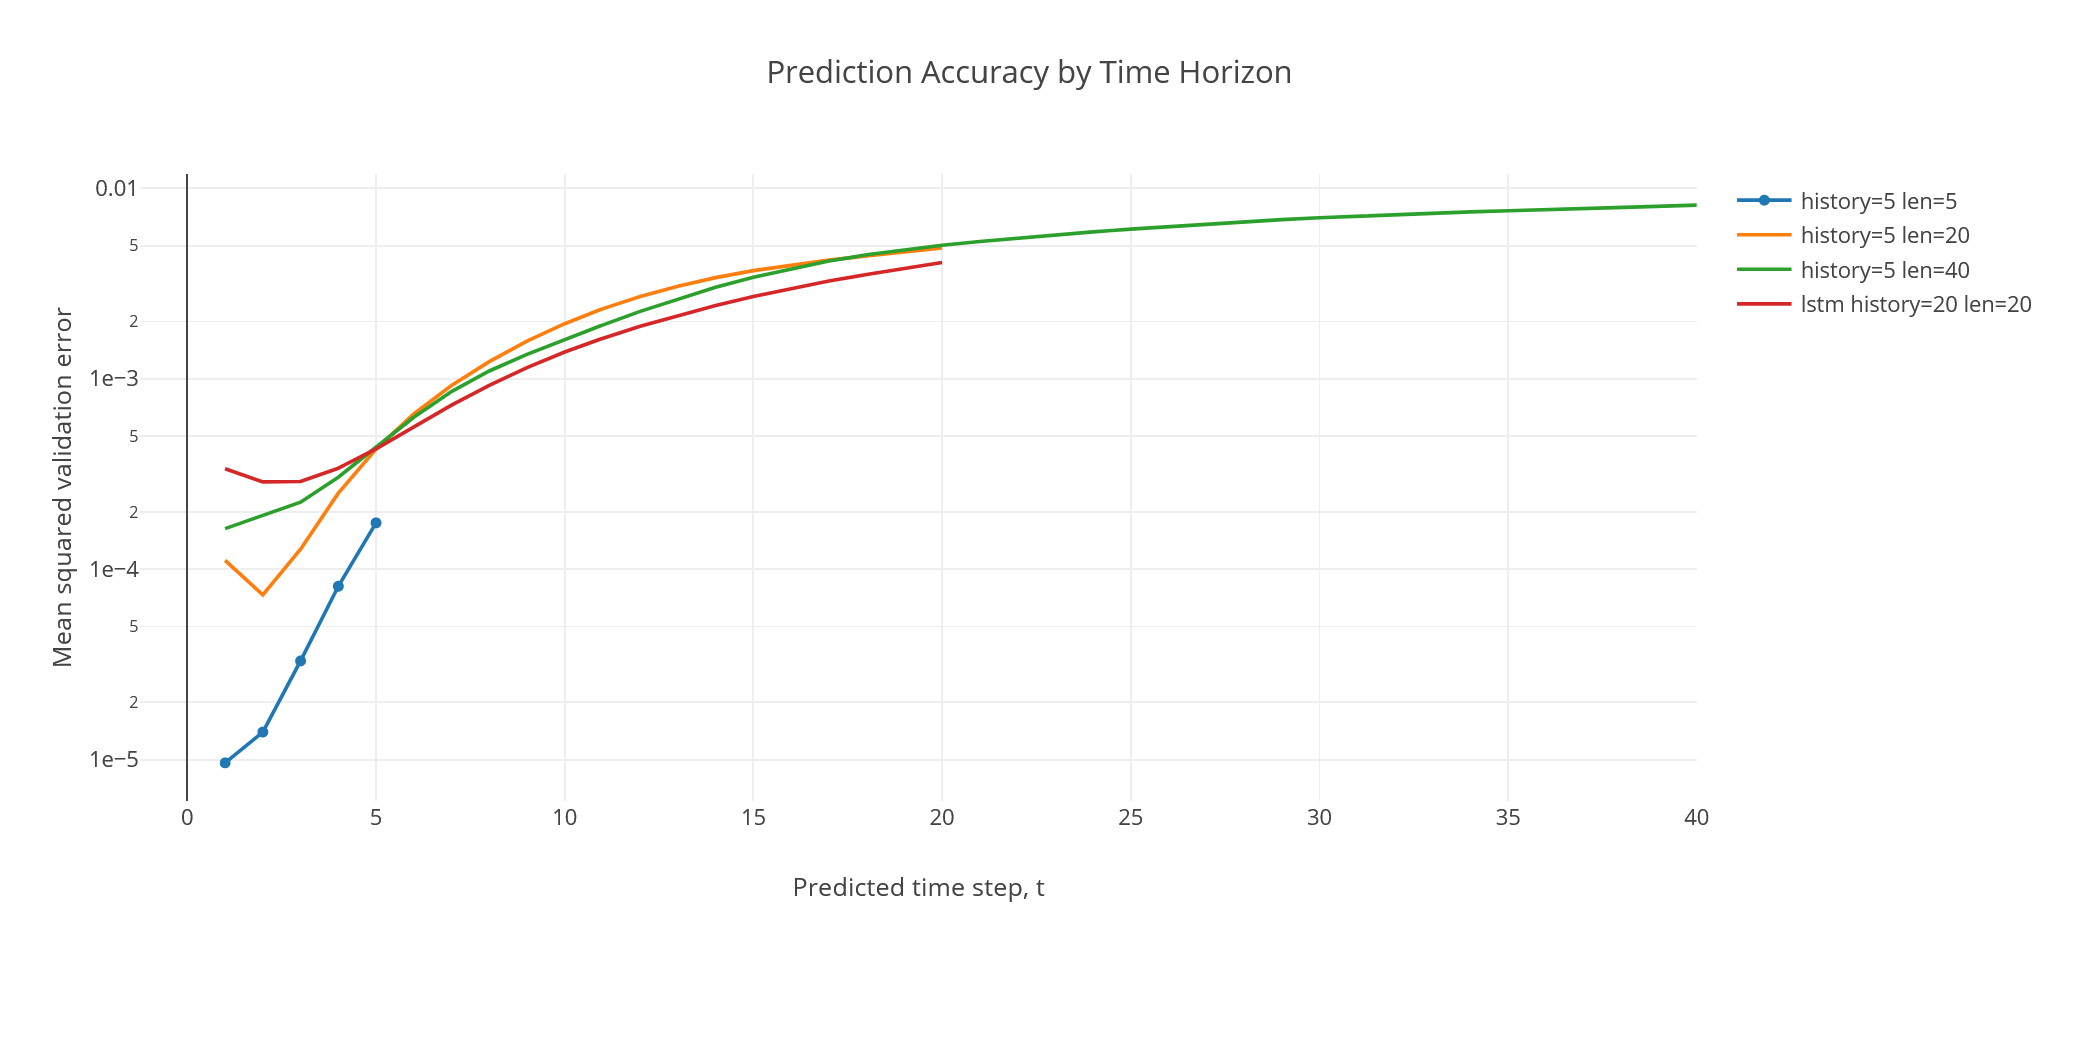
\includegraphics[width=0.9\linewidth]{pde_perf_linear}
        \caption{\small Performance of new PDE architecture for models trained trained using varying sequence lengths. Previous model LSTM model (in red) performs comparably to new model. The high accuracy shown by the short, 5-step prediction experiment suggests that compounding errors from edge effects are likely reducing long term prediction performance.}
        \label{fig:pdeperf}
    \end{figure}

    As shown in figure \ref{fig:pdeperf}, despite the simplified PDE architecture, the performance of the new models is comparable, being more accurate than the LSTM based model in the near-term samples and slightly less accurate in the long term. As illustrated by figures \ref{fig:pdeprediction} and \ref{fig:lstmprediction} the fully convolutional composition causes edge effects that reduce performance in long horizons as any assumptions made by local features valid in the center of the patch are violated when evaluated near the edges of the patch.

    \bibliographystyle{plain}
    \bibliography{}
    Sho Sonoda and Noboru Murata. Double continuum limit of deep neural networks.ICML WorkshopPrincipled Approaches to Deep Learning, 2017
\end{document}
